\documentclass[10pt]{beamer}

\usepackage{xeCJK}
\setCJKmainfont{Noto Sans CJK SC}
\xeCJKsetup{PunctStyle=kaiming,CJKspace=true,CheckSingle=true} 

\usepackage{subfigure}
\usepackage{amssymb, amsmath, amsfonts,verbatim}

\usepackage{tikz}

\graphicspath{ {./} }
\usetikzlibrary{matrix,arrows,fit,backgrounds,mindmap,plotmarks,decorations.pathreplacing}
\usepackage{tkz-euclide}
\usetkzobj{all}
\usepackage{pgfplots}
\pgfplotsset{compat=1.12}
\pgfdeclarelayer{background}
\pgfsetlayers{background,main}

\tikzset{decoration={name=none},}

\newlength\figureheight
\newlength\figurewidth

\newcommand{\tikzdir}[1]{#1.tikz}
\newcommand{\inputtikz}[1]{\input{\tikzdir{#1}}}

\newcommand{\tI}{\tilde {\mathcal I}}
\newcommand{\tA}{\tilde A}
\newcommand{\ty}{\tilde y}
\newcommand{\tx}{\tilde x}
\newcommand{\tw}{\tilde w}
\newcommand{\tv}{\tilde v}
\newcommand{\tC}{\tilde C}
\newcommand{\tP}{\tilde P}
\newcommand{\Ic}{{\mathcal I^c}}
\newcommand{\J}{{\mathcal J}}
\newcommand{\K}{{\mathcal K}}

\DeclareMathOperator{\Smin}{Smin}
\DeclareMathOperator{\Smid}{Smid}
\DeclareMathOperator{\Smax}{Smax}
\DeclareMathOperator{\MSE}{MSE}
\DeclareMathOperator{\rank}{rank}
\DeclareMathOperator{\Med}{Med}
\DeclareMathOperator{\Max}{Max}
\DeclareMathOperator{\Min}{Min}
\DeclareMathOperator{\tr}{tr}
\DeclareMathOperator{\Cov}{Cov}
\DeclareMathOperator{\logdet}{log\;det}
\DeclareMathOperator{\argmin}{arg\;min}
\DeclareMathOperator{\argmax}{arg\;max}
\let\Tiny\tiny

\title[Private Consensus]{分布式一致性问题中的隐私保护}
\author[Yilin Mo]{莫一林}
\institute[Tsinghua]{
  清华大学 自动化系
}
\date[Dec 5th, 2018]{Dec 5th, 2018}
  

\usetheme[subsectionpage=none,block=fill]{metropolis}
\definecolor{thupurple}{RGB}{102,8,116}
\definecolor{caltechcolor}{RGB}{102,8,116}
\setbeamercolor{title separator}{fg=black!50}
\setbeamercolor{frametitle}{bg=thupurple!70!black}
 

\begin{document}

\maketitle 
\section{An Illustrated Guide to a Ph.D.}

\begin{frame}{}
  Imagine a circle that contains all of human knowledge:

  \begin{figure}[hb]
    \centering
    
\includegraphics[width=0.8\textwidth]{images/PhDKnowledge-001.png}
  \end{figure}
\end{frame}


\begin{frame}{}
  By the time you finish elementary school, you know a little:
  \begin{figure}[hb]
    \centering
    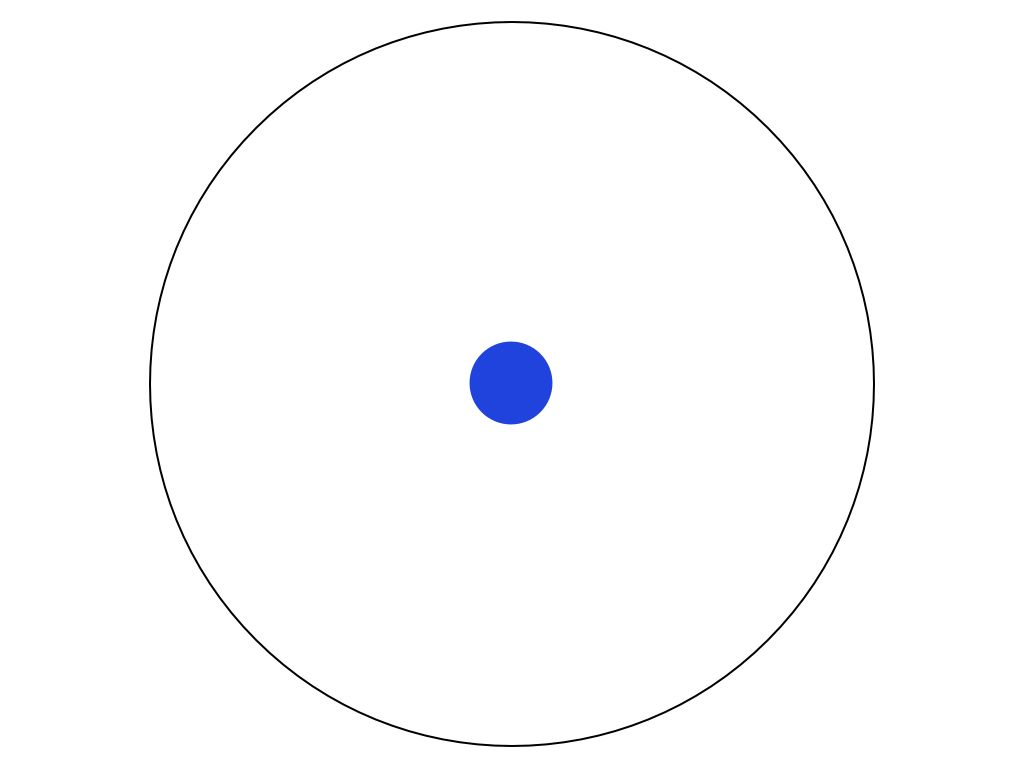
\includegraphics[width=0.8\textwidth]{images/PhDKnowledge-002.png}
  \end{figure}
\end{frame}


\begin{frame}{}
  By the time you finish high school, you know a bit more:
  \begin{figure}[hb]
    \centering
    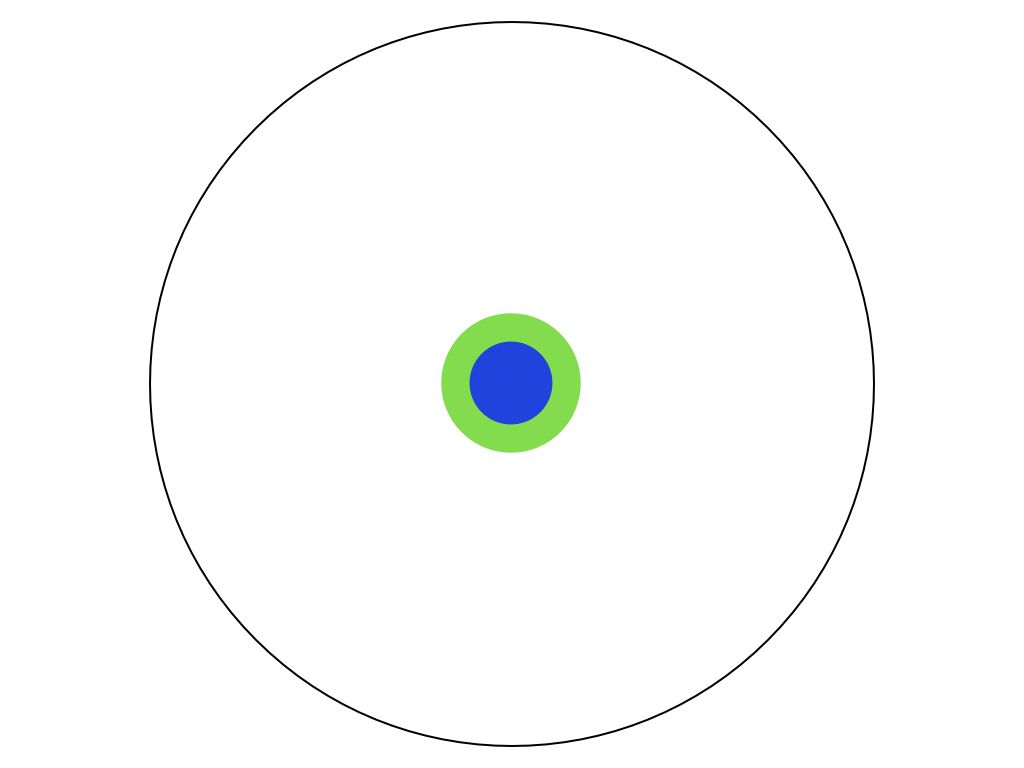
\includegraphics[width=0.8\textwidth]{images/PhDKnowledge-003.png}
  \end{figure}
\end{frame}


\begin{frame}{}
  With a bachelor's degree, you gain a specialty:
  \begin{figure}[hb]
    \centering
    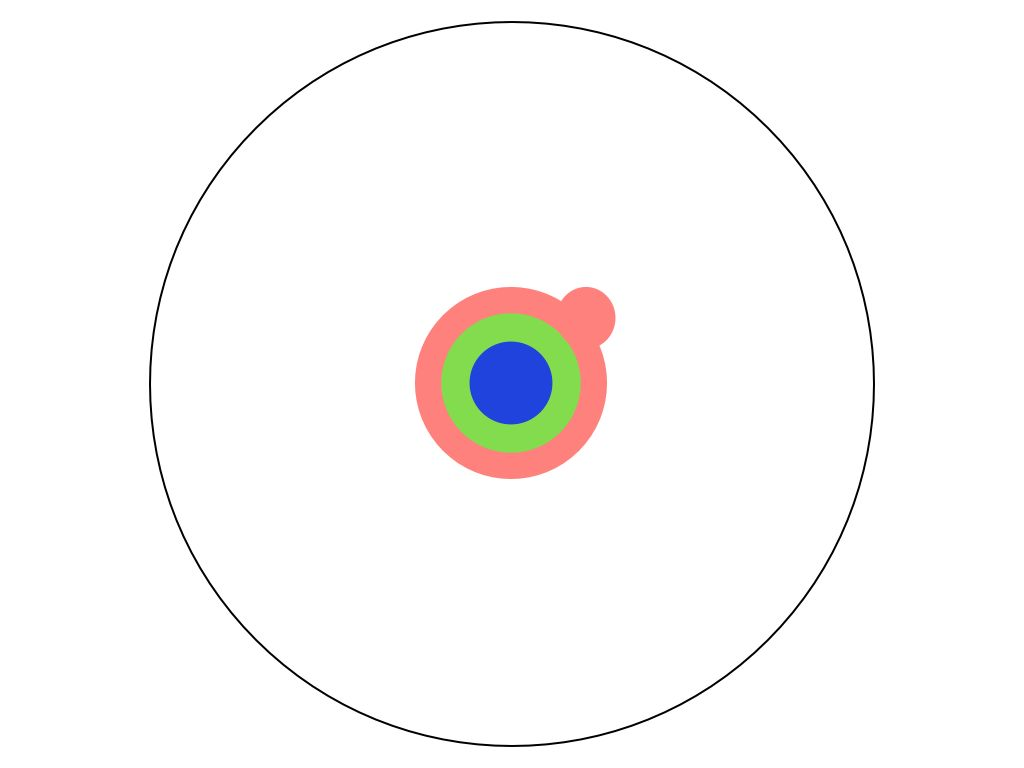
\includegraphics[width=0.8\textwidth]{images/PhDKnowledge-004.png}
  \end{figure}
\end{frame}



\begin{frame}{}
  A master's degree deepens that specialty:
  \begin{figure}[hb]
    \centering
    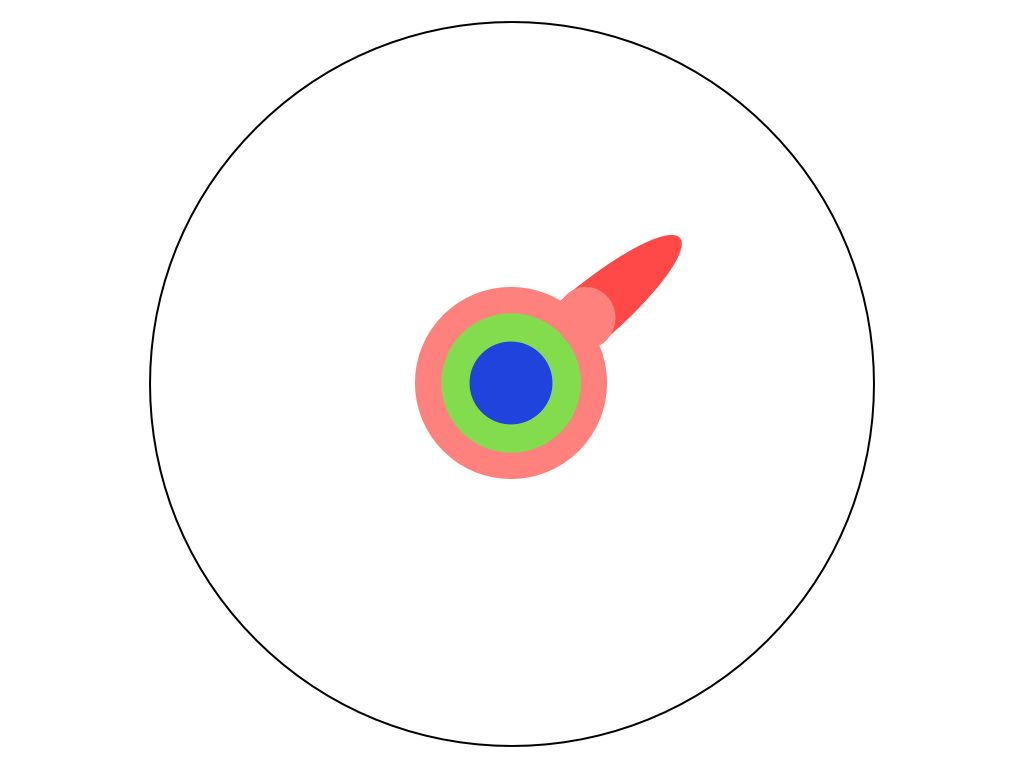
\includegraphics[width=0.8\textwidth]{images/PhDKnowledge-005.png}
  \end{figure}
\end{frame}



\begin{frame}{}
  Reading research papers takes you to the edge of human knowledge:
  \begin{figure}[hb]
    \centering
    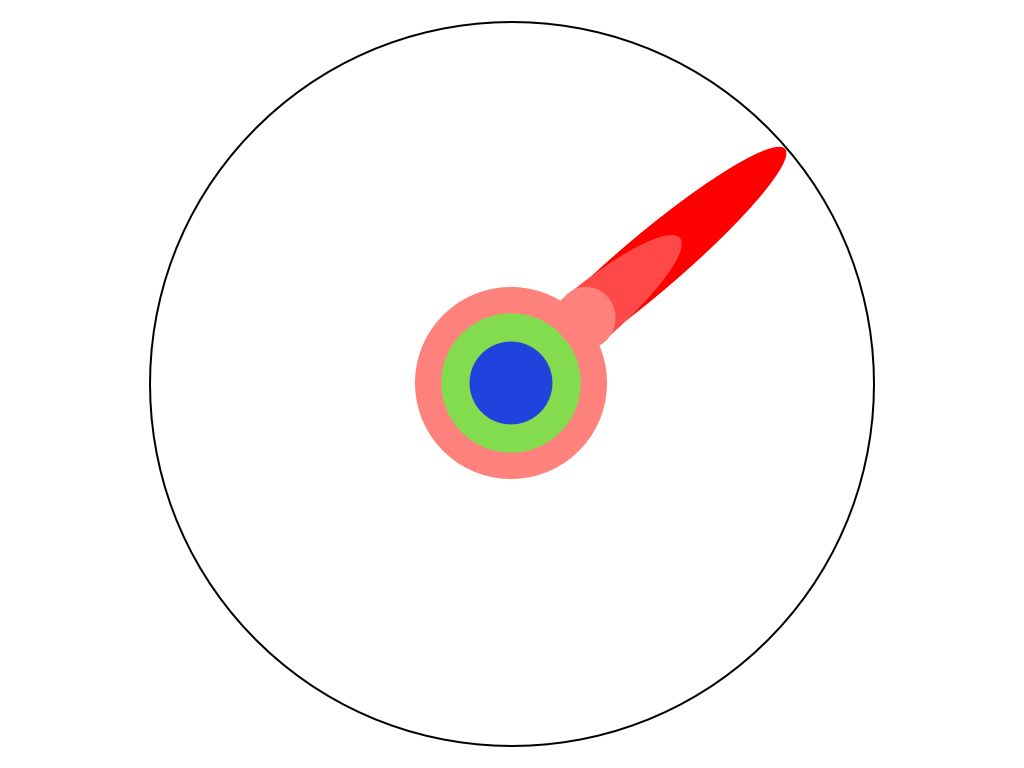
\includegraphics[width=0.8\textwidth]{images/PhDKnowledge-006.png}
  \end{figure}
\end{frame}


\begin{frame}{}
  Once you're at the boundary, you focus:
  \begin{figure}[hb]
    \centering
    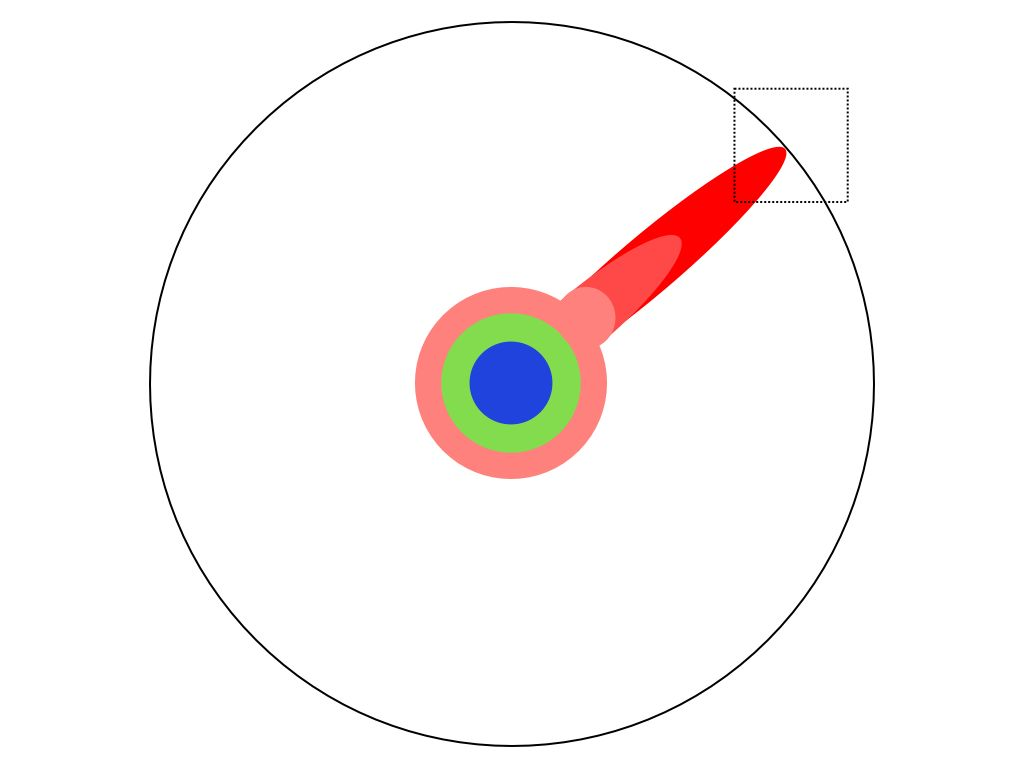
\includegraphics[width=0.8\textwidth]{images/PhDKnowledge-007.png}
  \end{figure}
\end{frame}


\begin{frame}{}
  You push at the boundary for a few years:
  \begin{figure}[hb]
    \centering
    
\includegraphics[width=0.8\textwidth]{images/PhDKnowledge-008.png}
  \end{figure}
\end{frame}

\begin{frame}{}
  Until one day, the boundary gives way:
  \begin{figure}[hb]
    \centering
    
\includegraphics[width=0.8\textwidth]{images/PhDKnowledge-009.png}
  \end{figure}
\end{frame}


\begin{frame}{}
  And, that dent you've made is called a Ph.D.:

  \begin{figure}[hb]
    \centering
    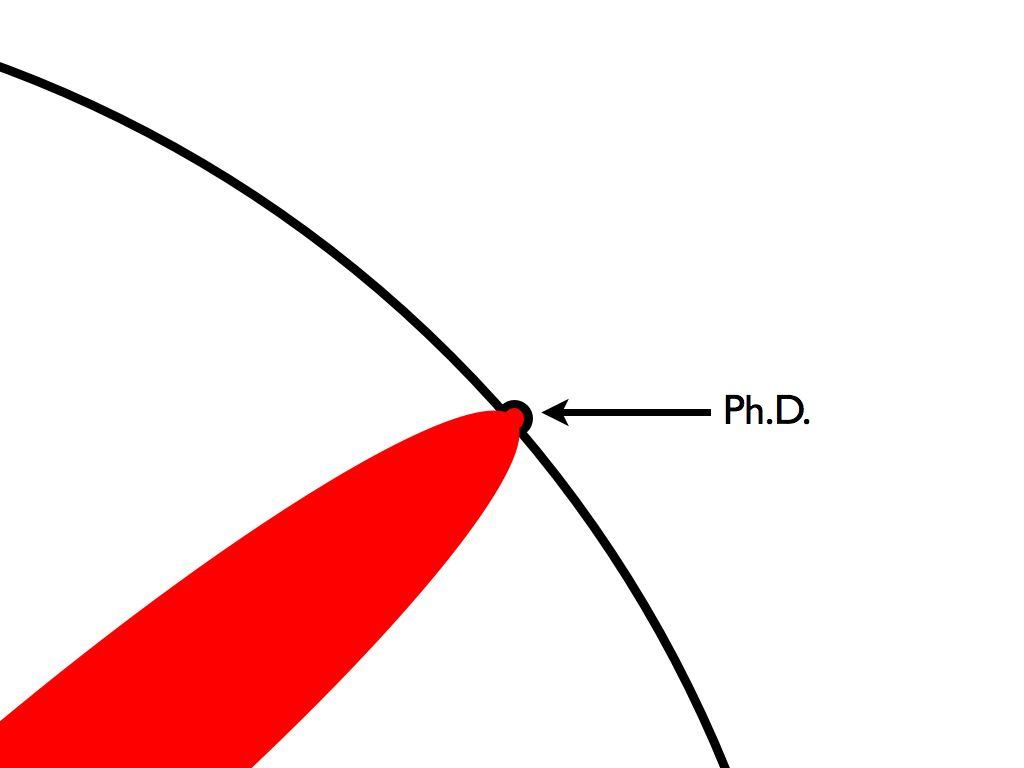
\includegraphics[width=0.8\textwidth]{images/PhDKnowledge-010.png}
  \end{figure}
\end{frame}


\begin{frame}{}
  Of course, the world looks different to you now:
  \begin{figure}[hb]
    \centering
    
\includegraphics[width=0.8\textwidth]{images/PhDKnowledge-011.png}
  \end{figure}
\end{frame}


\begin{frame}{}
  So, don't forget the bigger picture:
  \begin{figure}[hb]
    \centering
    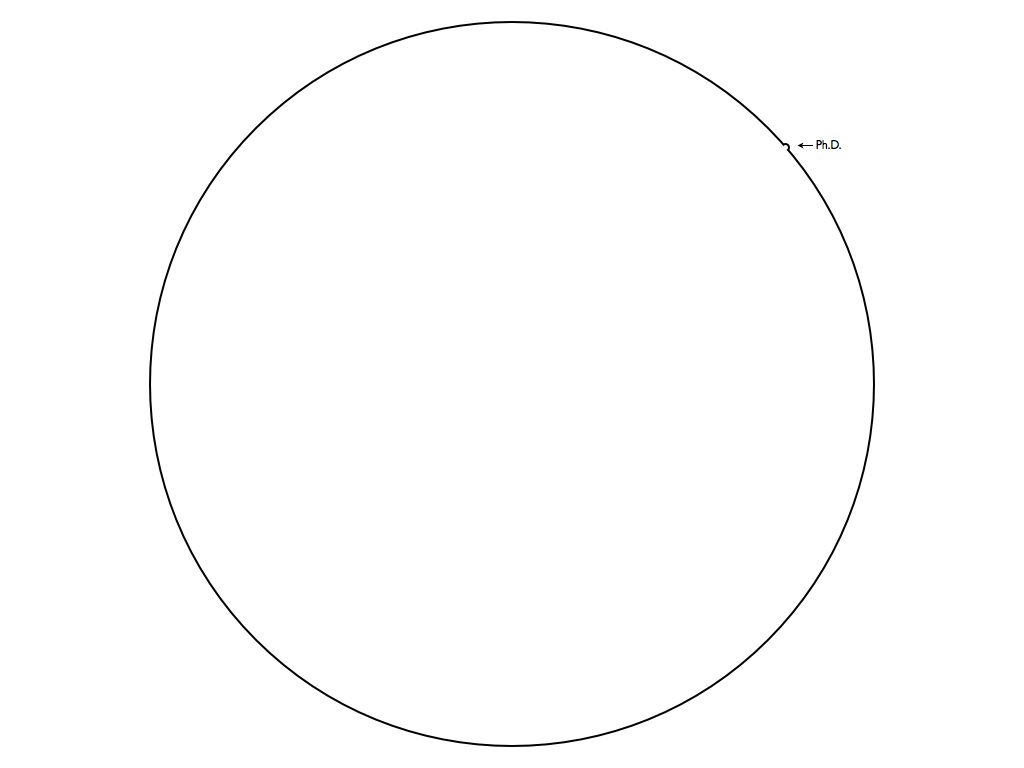
\includegraphics[width=0.8\textwidth]{./images/PhDKnowledge-012.png}
  \end{figure}
\end{frame}

\begin{frame}{}
  \Huge Keep pushing.
\end{frame}

\begin{frame}{信息物理系统}
  \begin{itemize}
  \item Cyber-Physical Systems (CPSs) refer to the embedding of computation, communication and control into physical spaces.
    \begin{center}
      \begin{tikzpicture}[scale=0.45,transform shape,level distance=0cm,
        level 1 concept/.append style={sibling angle=120,minimum size = 3cm},
        ]
        \path [draw=thupurple!50,fill=thupurple!20,thick,rounded corners] (-10,-4.5) rectangle (10,7);
        \node at (-9,6) [anchor=north west] {\Huge 物理空间};
        \path[mindmap,concept color=black,text=white]
        node[concept] {\Huge CPS}
        [clockwise from=330]
        child[concept color=green!50!black] { node[concept](communication) {\huge 通讯} }
        child[concept color=red] { node[concept](control) {\huge 控制} }
        child[concept color=blue] { node[concept](computation) {\huge 计算} };
      \end{tikzpicture}
    \end{center}
  \item Applications: aerospace, chemical processes, civil infrastructure, energy, manufacturing and transportation. 
  \end{itemize}
\end{frame}

\begin{frame}{Stuxnet}
  \begin{figure}[ht]
    \centering
    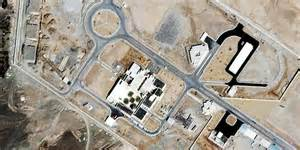
\includegraphics[width=0.8\textwidth]{stuxnet.jpg}
  \end{figure}
  Stuxnet is the first discovered malware that spies on and subverts industrial control systems. It was discovered in June 2010. 
\end{frame}

\begin{frame}{Industrial Control Systems}
  \begin{figure}[ht]
    \centering
    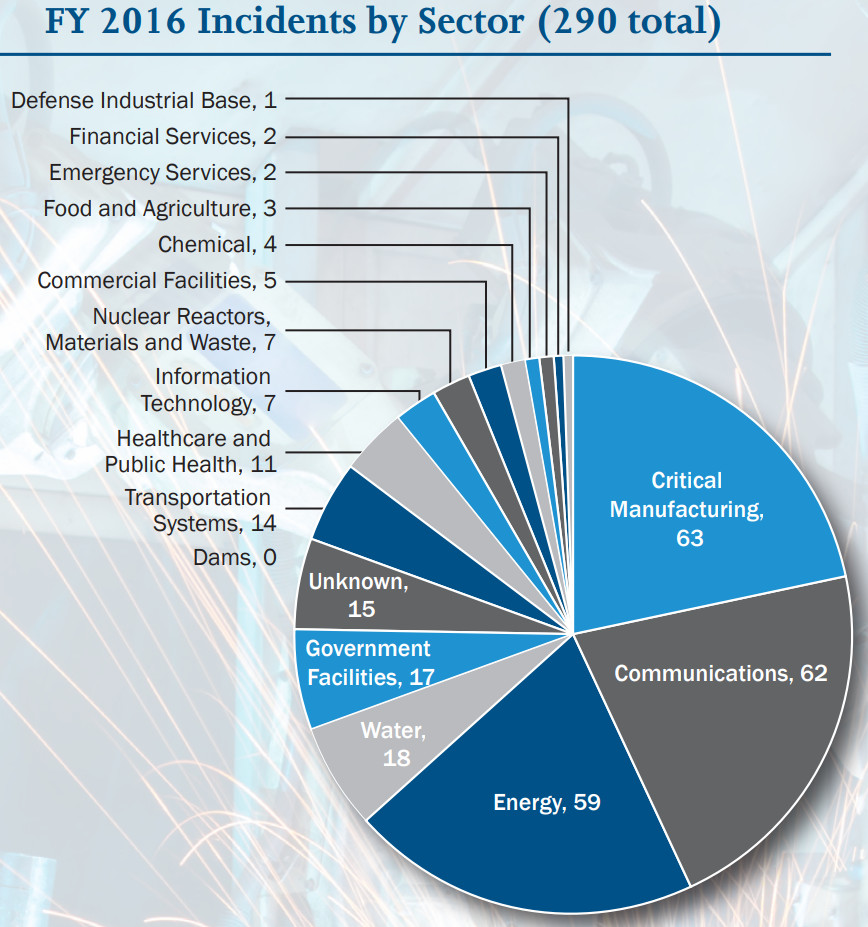
\includegraphics[width=0.6\textwidth]{cert.jpg}
  \end{figure}
  In FY 2014, ICS-CERT (Industrial Control Systems Cyber Emergency Response Team) received and responded to 245 incidents as reported by asset owners and industry partners. This number increased to 290 in FY 2016.
\end{frame}

\begin{frame}[standout]
  感谢各位老师同学聆听,请大家批评指正!
\end{frame}

\end{document}

%%% Local Variables: 
%%% coding: utf-8
%%% mode: latex
%%% TeX-engine: xetex
%%% End: 